%\documentclass{sig-alternate}
\documentclass{llncs}
\usepackage{amsmath,amssymb,graphicx}
\usepackage[ruled,linesnumbered]{algorithm2e}
\usepackage{algorithmic}
\usepackage{mdwlist}
\usepackage{color}
\usepackage{multirow}
\usepackage{rotating}
\usepackage{slashbox}
\usepackage{amsmath}
\usepackage[mathscr]{eucal} %% For \mathscr
\usepackage{amsbsy} %% For \boldsymbol
\newcommand{\T}[1]{\boldsymbol{\mathscr{#1}}}  
\usepackage{subfigure}
\usepackage{booktabs}
\usepackage{tikz}
\usetikzlibrary{snakes}
\usepackage{multirow}
\usepackage{epstopdf}
\usepackage{enumitem}
\usepackage{url}
\usepackage{array}
\setlist{nolistsep}
\newcommand{\hide}[1]{}
\usepackage[labelfont=bf]{caption}
\DeclareCaptionType{copyrightbox}
\DeclareMathOperator*{\argmin}{argmin}
\DeclareMathOperator*{\argmax}{argmax}
\newcommand{\reminder}[1]{ {\color{red} {\bf  #1} } }
\newcommand{\BigO}[1]{\ensuremath{\operatorname{O}\bigl(#1\bigr)}}

\title{Binomial and Fibonacci Heaps in Racket (rkt-heaps)}

\begin{document}

\author{
	Abhinav Jauhri\\
	\texttt{abhinavjauhri@gmail.com}\\
}


% The \author macro works with any number of authors. There are two commands
% used to separate the names and addresses of multiple authors: \And and \AND.
%
% Using \And between authors leaves it to \LaTeX{} to determine where to break
% the lines. Using \AND forces a linebreak at that point. So, if \LaTeX{}
% puts 3 of 4 authors names on the first line, and the last on the second
% line, try using \AND instead of \And before the third author name.

%\newcommand{\fix}{\marginpar{FIX}}
%\newcommand{\new}{\marginpar{NEW}}

%\nipsfinalcopy % Uncomment for camera-ready version


\maketitle
%\vspace{-0.5in}

\begin{abstract}
	Library\footnote{Will be referred as $rkt-heaps$ throughout the paper} providing data structures viz. Binomial heap \cite{vuillemin1978data} and Fibonacci heap\cite{fredman1987fibonacci} are described along with primitive operations, performance and usage. 
\end{abstract}

\section{Introduction}
%\vspace{-0.1in}
$rkt-heaps$ library is made for demonstration in a contest, \textit{Lisp In Summer Projects}\footnote{http://lispinsummerprojects.org/}. The goals of any participating individual in the contest were to build and demonstrate a project using any LISP-based technology. $rkt-heaps$ uses Racket language belonging to the Lisp/Scheme family. \\

\emph{Section 1 \& 2} describe Binomial and Fibonacci heaps respectively. \emph{Section 3} has performance results to complement the theoretical run-time bounds. Comparison with an existing library for Binary heaps\footnote{http://docs.racket-lang.org/data/Binary\_Heaps.html} in Racket is also added for evaluation purposes. \emph{Section 4} talks about syntactics of using this library in Racket.

\section{Binomial Heaps}
Binomial heaps are a collection of heap-ordered Binomial trees with a pointer $min$ to the root of a tree having the minimum value amongst all elements in the heap. They allow the following operations: \\

\begin{enumerate}
	\item \emph{makeheap(i)} Makes a new heap with only one element \emph{i}.
	\item \emph{findmin(h)} Returns the minimum value amongst all elements in the heap.
	\item \emph{insert(h, i)} Adds element \emph{i} to heap \emph{h}
	\item \emph{deletemin(h)} Deletes the element with minimum value from \emph{h}
	\item \emph{meld(h, h')} Combines two heaps \emph{h} and \emph{h'} into one \\
\end{enumerate}

\begin{table}
	\centering
	\begin{tabular}{| >{\centering\arraybackslash}m{1in} | >{\centering\arraybackslash}m{1in} |}
		\hline
		\centering
		Operation & Amortized Cost \\ 
		\hline
		makeheap & \BigO{1}    \\
		findmin & \BigO{1} \\ 
		insert & \BigO{1}  \\
		deletemin & \BigO{\log n} \\
		meld (eager) & \BigO{\log n}\\
		meld (lazy) & \BigO{1} \\ \hline
	\end{tabular}
	\caption{Amortized costs for Binomial Heaps}
	\label{tab:binomialcost}
\end{table}

Amortized cost may not always give the exact cost of an operation. An operation may be expensive or cheaper, but the average cost over a sequence of operations is small. Another, relevant term for study of such heaps is $rank$. It states the number of children of a node. For Binomial and Fibonacci heaps, only when no $decrement$ and $delete$ operations are performed, the rank of a root node is $k$ with $2^k$ nodes.

Making a new heap with one element $makeheap$ and finding the $min$ pointer to get the minimum value requires constant number of steps. It is not intuitive to see why $insert$ takes just constant amortized time. Inserting a value is interpreted as making a heap with a single element and then merging it with the existing heap. In melding, combining two trees with same rank $k$ leads to a tree of rank $k+1$. If one already exists in either of the heaps, then a tree of rank $k+2$ is made. This happens recursively till there is single tree of some rank $(>k)$ in the resulting heap. Each time trees are combined, the heap property is imposed i.e. the minimum between the two roots becomes the root of the combined tree. This make the average cost over $n$ operations to be \BigO{1} for $insert$. Similarly, the combining of roots of trees can be extended for $deletemin$ operation. Take all children of the min root and meld them with the remaining trees in the heap, and update the min pointer, costing \BigO{\log n}.

$meld$ eager version works in the manner as described above but for the lazy version, all roots of one heap are added to the set of roots of the other heap. This may result in having more than one binomial tree of rank $k$ in the resulting heap. Subsequent call to a $deletemin$ operation will correct the heap such that only one binomial tree of rank $k$ exists. This costs \BigO{\log n}.

Binomial heaps is $rkt-heaps$ is an array-based purely functional implementation. Specifically using Racket's $vectors$ library. Being purely functional ensures there is no mutation of previously created data structures. Although, this leads to anomalies in runtime costs for certain operations like \emph{insert}. With reference to Table \ref{tab:binomialcost}, the total cost for $n$ inserts is linear, \BigO{n}; but in a purely functional implementation, the insert operation cost for $n$ inserts aggregates to \BigO{n^2}. The reason for such an anomaly is due to cloning of heap vector at every insert operation. This is validated in Fig:\ref{fig:bino_anomaly}. The curve \emph{binomial-insert (linear)} signifies the divisor(amortized cost) for the dividend(average cost) is linear in $n$, and therefore the curve has slope zero. Alternatively, taking the divisor as constant, the average run-time cost depicts a linear increase in cloning the vector, which is to say that $nth$ insertion step clones the $(n-1)th$ heap vector\footnote{Racket's vector API provides \emph{(vector-append v\_1 v\_2 \dots)}, used for cloning, makes fresh copy of all elements of the given vectors}. Modifying the structuring of the heap to a doubly linked list(DDL) is imperative to ensure constant number of steps for each insert (used for analyzing run-time costs in \cite{kozen1992design}). The DDL implementation and cost shall be discussed in later sections of this paper. The array implementation was done out of pedagogical curiosity of the author.

\begin{figure}
\begin{center}
	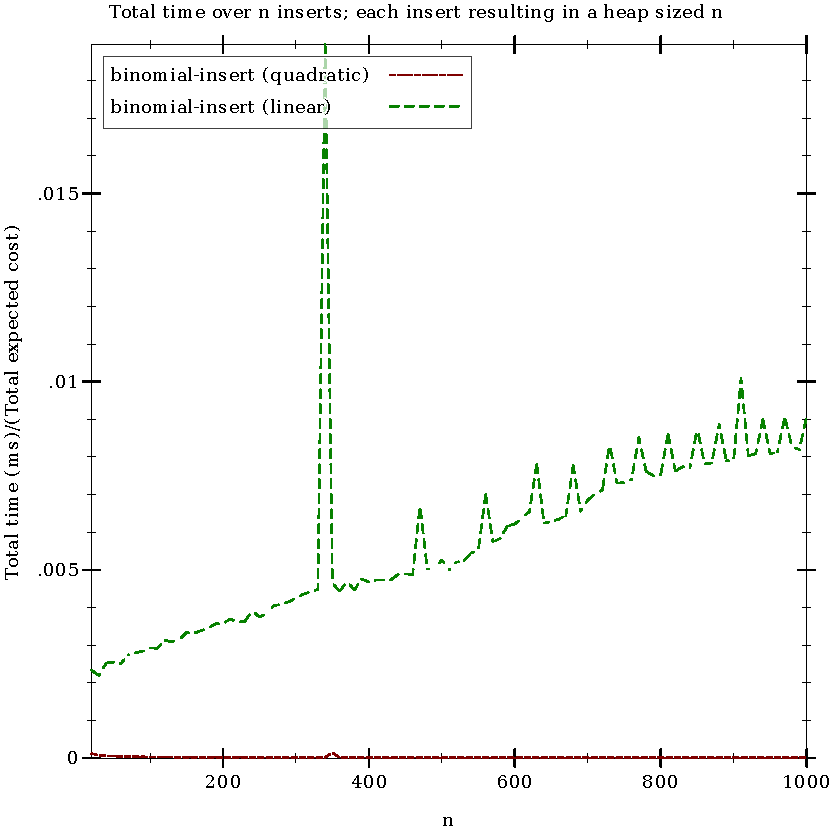
\includegraphics[width=0.8\textwidth]{FIG/insert_binomial.pdf}
\end{center}
\caption{Anomaly in $insert$ operations for Binomial heaps. The y-axis shows the (average runtime cost)/(amortized cost). For one curve it is linear in $n$, and for the other it is just a constant. By average, it means over $n$ insert operations and maintaining the heap state in-between inserts}
\label{fig:bino_anomaly}
\end{figure}

\section{Fibonacci Heaps}
Fibonacci heaps are a generalization of Binomial heaps allowing additional operations other than those in Binomial heaps. Specifically, they allow deletion of an element from the heap, and modification of the value of an element. The prototypes for additional operations are as follows: \\

\begin{enumerate}
	\item \emph{decrement(h, i, $\delta$)} Decrements the value of $i$ by $\delta$ in $h$
	\item \emph{delete(h, i)} Deletes element $i$ from the heap $h$ 
\end{enumerate}

\begin{table}
	\centering
	\begin{tabular}{| >{\centering\arraybackslash}m{1in} | >{\centering\arraybackslash}m{1in} |}
		\hline
		\centering
		Operation & Amortized Cost \\ 
		\hline
		\rule{0pt}{3ex}makeheap & \BigO{1}    \\
		findmin & \BigO{1} \\ 
		insert & \BigO{1}  \\
		deletemin & \BigO{\log n} \\
		meld (lazy) & \BigO{1} \\ 
		decrement & \BigO{1} \\
		delete & \BigO{\log n}\\ \hline
	\end{tabular}
	\caption{Amortized costs for Fibonacci Heaps}
	\label{tab:fibonaccicost}
\end{table}

Fibonacci heaps are implemented in $rkt-heaps$ using a DDL based on the learnings from the array based implementation of Binomial heaps. As stated earlier that in a Fibonacci heap only $deletemin$ and $meld$ operations are consdiered, then every tree becomes a binomial tree, thus ensuring the size of tree rooted at $r$ to be exponential in $rank(r)$. This is also valid for Fibonacci heaps with operations like $decrement$ and $delete$ \cite{kozen1992design}.

$decrement$ operation after chaning the value of an element, check whether the heap propoerty is violated or not. If it is, then the sub-tree rooted at that element, is added to the DDDL of root of the heap. Ever element has a flag marked as true if one of its children have been cut or deleted. This element if makred and another child is cut, the lement is also added to the DDL of roots of theheap.





\section{Evaluation}


\section{Usage}

\section{Conclusion}

%\newpage
\bibliographystyle{plain}
\bibliography{BIB/refs.bib}

\end{document}
